\documentclass[tikz,border=14pt]{standalone}
\usepackage[T1]{fontenc}
\usepackage{tgheros}
\renewcommand*\familydefault{\sfdefault}
\usepackage{pgfplots}
\pgfplotsset{compat=1.18}
\usepgfplotslibrary{fillbetween}
\usetikzlibrary{arrows.meta, calc}
\pgfdeclarelayer{background}
\pgfsetlayers{background,main}
\newcommand{\toyCliffA}{99.9000}\newcommand{\toyCliffAL}{99.9}
\newcommand{\toyCliffB}{71.5000}\newcommand{\toyCliffBL}{71.5}
\newcommand{\toyCliffC}{3.6667}\newcommand{\toyCliffCL}{3.7}
\newcommand{\toyCliffD}{1.6333}\newcommand{\toyCliffDL}{1.6}
\newcommand{\realCliffA}{84.5000}\newcommand{\realCliffAL}{84.5}
\newcommand{\realCliffB}{51.0000}\newcommand{\realCliffBL}{51.0}
\newcommand{\realCliffC}{6.5000}\newcommand{\realCliffCL}{6.5}
\newcommand{\toyAttA}{0.7122}\newcommand{\toyAttAL}{0.71}
\newcommand{\toyAttB}{0.4090}\newcommand{\toyAttBL}{0.41}
\newcommand{\toyAttC}{0.1179}\newcommand{\toyAttCL}{0.12}
\newcommand{\toyAttD}{0.0241}\newcommand{\toyAttDL}{0.02}
\newcommand{\realAttIn}{0.4632}\newcommand{\realAttInL}{0.46}
\newcommand{\realAttFar}{0.1077}\newcommand{\realAttFarL}{0.11}
\newcommand{\realHeads}{39.0000}\newcommand{\realHeadsL}{39}
\newcommand{\toyNone}{1.6667}\newcommand{\toyNoneL}{1.7}
\newcommand{\realTwoNone}{51.0000}\newcommand{\realTwoNoneL}{51.0}
\newcommand{\realFourNone}{6.5000}\newcommand{\realFourNoneL}{6.5}
\newcommand{\toyPatch}{76.1500}\newcommand{\toyPatchL}{76.1}
\newcommand{\realTwoPatch}{85.5000}\newcommand{\realTwoPatchL}{85.5}
\newcommand{\realFourPatch}{65.0000}\newcommand{\realFourPatchL}{65.0}
\newcommand{\toySham}{1.2833}\newcommand{\toyShamL}{1.3}
\newcommand{\realTwoSham}{1.0000}\newcommand{\realTwoShamL}{1.0}
\newcommand{\realFourSham}{1.0000}\newcommand{\realFourShamL}{1.0}
\newcommand{\realFourPatchFull}{25.5000}\newcommand{\realFourPatchFullL}{25.5}
\newcommand{\bestFixAnywhere}{9.3333}\newcommand{\bestFixAnywhereL}{9.3}
\newcommand{\fixMaxFar}{1.4333}\newcommand{\fixMaxFarL}{1.4}
\newcommand{\auditToyNone}{1.5833}\newcommand{\auditToyNoneL}{1.6}
\newcommand{\auditToyPatch}{75.6667}\newcommand{\auditToyPatchL}{75.7}
\newcommand{\auditTwoNone}{55.5556}\newcommand{\auditTwoNoneL}{55.6}
\newcommand{\auditTwoPatch}{100.0000}\newcommand{\auditTwoPatchL}{100.0}
\newcommand{\auditTwoN}{18.0000}\newcommand{\auditTwoNL}{18}
\newcommand{\marginOrig}{0.6780}\newcommand{\marginOrigL}{0.68}
\newcommand{\marginAudit}{1.1240}\newcommand{\marginAuditL}{1.12}


\definecolor{ink}{HTML}{0B0B0B}
\definecolor{muted}{HTML}{6B6A66}
\definecolor{gridc}{HTML}{E6E5E0}
\definecolor{band}{HTML}{F3F2EE}
\definecolor{cnone}{HTML}{52514E}
\definecolor{cpatch}{HTML}{2A78D6}
\definecolor{csham}{HTML}{008300}
\definecolor{corange}{HTML}{EB6834}
\definecolor{softblue}{HTML}{CFE1F7}
\definecolor{softgray}{HTML}{C9C8C2}

\newcommand{\pct}[1]{#1\%}

\pgfplotsset{
  /pgf/number format/assume math mode=true,
  base/.style={
    axis line style={muted, line width=0.4pt},
    tick style={muted, line width=0.4pt},
    tick align=outside,
    axis x line*=bottom, axis y line*=left,
    every tick label/.append style={font=\small, text=muted},
    label style={font=\small, text=muted},
    grid=major, major grid style={gridc, line width=0.4pt},
    title style={font=\normalsize\bfseries, text=ink},
    clip=false,
  },
}
\tikzset{
  figtitle/.style={font=\LARGE\bfseries, text=ink, anchor=north west, inner sep=0pt},
  figsub/.style={font=\normalsize, text=muted, anchor=north west, align=left, text width=17cm, inner sep=0pt, execute at begin node={\hyphenpenalty=10000\exhyphenpenalty=10000}},
  footnote/.style={font=\small, text=muted, anchor=north west, align=left, text width=17cm, inner sep=0pt, execute at begin node={\hyphenpenalty=10000\exhyphenpenalty=10000}},
  big/.style={font=\Large\bfseries, inner sep=2pt},
  lab/.style={font=\small, text=ink, inner sep=2pt},
  quiet/.style={font=\small, text=muted, inner sep=2pt},
}
\newcommand{\header}[2]{\node[figtitle] (title) at (0,0) {#1};
  \node[figsub] (sub) at ($(title.south west)+(0,-8pt)$) {#2};}

  \pgfplotsset{cliff/.style={base, height=6.4cm, log basis x=2, xmin=1, ymin=0, ymax=100,
    ytick={0,50,100}, yticklabels={0\%,50\%,100\%}, xmajorgrids=false, axis on top,
    xlabel={input length, in multiples of the trained length}}}
\begin{document}
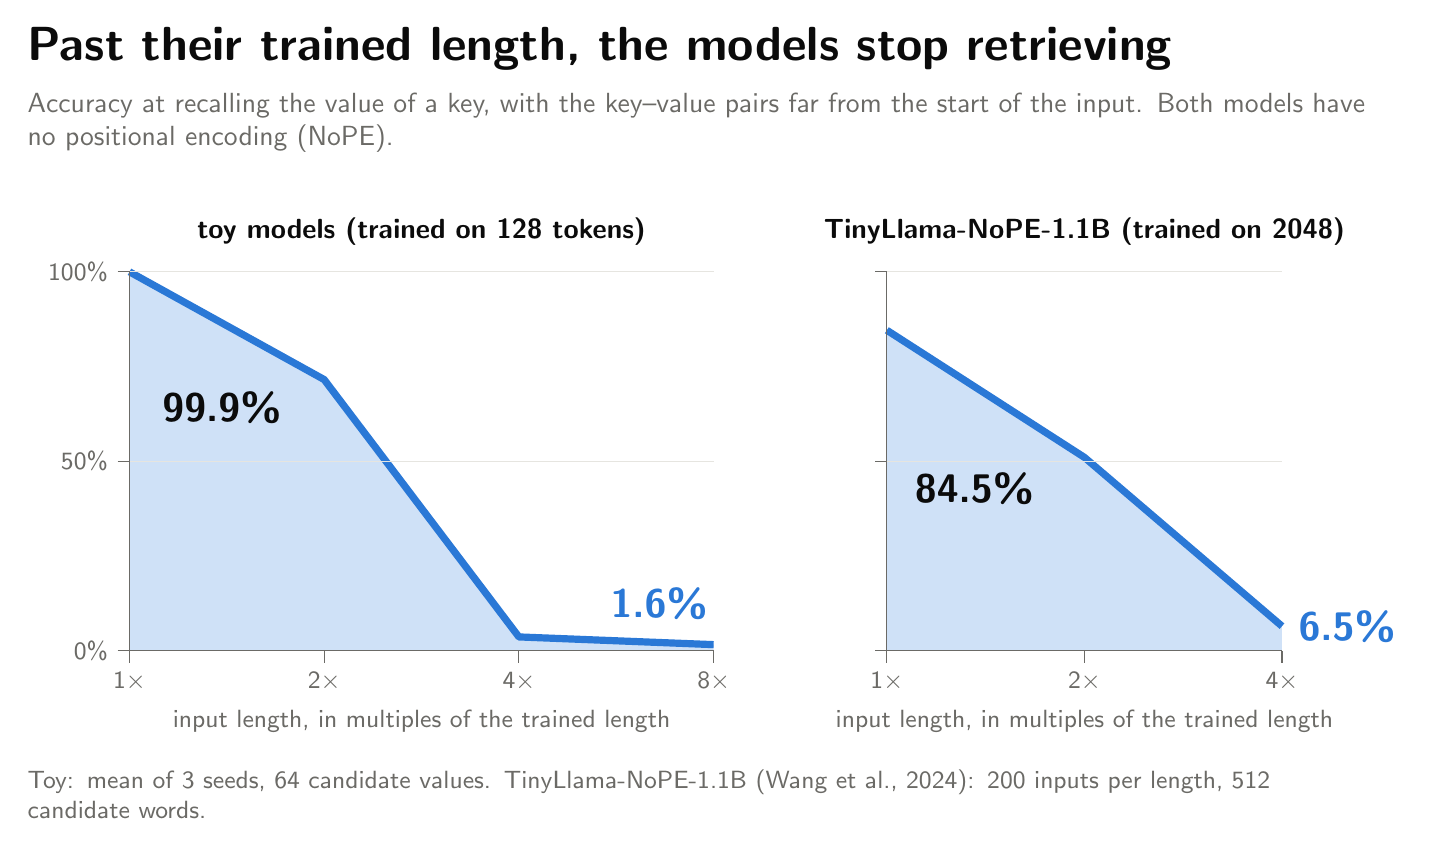
\begin{tikzpicture}
  \header{Past their trained length, the models stop retrieving}
    {Accuracy at recalling the value of a key, with the key--value pairs far from the start of the input.
     Both models have no positional encoding (NoPE).}

  \begin{axis}[cliff, xmode=log, name=toy, at={($(sub.south west)+(1.3cm,-1.5cm)$)}, anchor=north west, width=9.0cm,
      xmax=8, xtick={1,2,4,8}, xticklabels={1$\times$,2$\times$,4$\times$,8$\times$},
      title={toy models (trained on 128 tokens)}]
    \addplot[draw=none, fill=softblue] coordinates
      {(1,\toyCliffA) (2,\toyCliffB) (4,\toyCliffC) (8,\toyCliffD)} \closedcycle;
    \addplot[cpatch, line width=2.6pt, line join=round] coordinates
      {(1,\toyCliffA) (2,\toyCliffB) (4,\toyCliffC) (8,\toyCliffD)};
    \node[big, text=ink, anchor=north west] at (axis cs:1.1,\toyCliffA - 30) {\pct{\toyCliffAL}};
    \node[big, text=cpatch, anchor=south east] at (axis cs:8,\toyCliffD + 5) {\pct{\toyCliffDL}};
  \end{axis}

  \begin{axis}[cliff, xmode=log, name=real, at={($(toy.north east)+(2.2cm,0)$)}, anchor=north west, width=6.6cm,
      xmax=4, xtick={1,2,4}, xticklabels={1$\times$,2$\times$,4$\times$}, yticklabels={},
      title={TinyLlama-NoPE-1.1B (trained on 2048)}]
    \addplot[draw=none, fill=softblue] coordinates {(1,\realCliffA) (2,\realCliffB) (4,\realCliffC)} \closedcycle;
    \addplot[cpatch, line width=2.6pt, line join=round] coordinates {(1,\realCliffA) (2,\realCliffB) (4,\realCliffC)};
    \node[big, text=ink, anchor=north west] at (axis cs:1.08,\realCliffA - 36) {\pct{\realCliffAL}};
    \node[big, text=cpatch, anchor=west] at (axis cs:4.15,\realCliffC) {\pct{\realCliffCL}};
  \end{axis}

  \node[footnote] at ($(toy.south west)+(-1.3cm,-1.5cm)$) {Toy: mean of 3 seeds, 64 candidate values.
    TinyLlama-NoPE-1.1B (Wang et al., 2024): 200 inputs per length, 512 candidate words.};
\end{tikzpicture}
\end{document}
